\subsection{Кейс-стаді КДПУ: три програми дизайну поглиблено}\label{subsec:2.2}

Загальнонаціональний аналіз (п.~\ref{subsec:2.1}) виявив системну прогалину у формуванні ІКК на макрорівні. Для поглибленого розуміння стану ІКК-спрямованого змісту на інституційному рівні проведено кейс-стаді трьох освітніх програм спеціальності 022~Дизайн Криворізького державного педагогічного університету (КДПУ): <<Графічний дизайн>> (ГД), <<Дизайн одягу>> (ДО) та <<Дизайн середовища>> (ДС).

\subsubsection{Еволюція навчальних програм 2017--2021}\label{sssec:2.2.1}

У 2017--2018~рр. КДПУ пропонував єдину ОПП <<Дизайн>>. У 2019~р. відбулася диференціація на три окремі програми, які були оновлені у 2021~р. Для відстеження еволюції ІКК-спрямованого змісту проведено аналіз 8 версій ОПП (2017, 2018, ГД/ДО/ДС 2019, ГД/ДО/ДС 2021) із застосуванням автоматизованого підрахунку ІКК-ключових слів за 4 компонентами.

\begin{table}[htbp]
\centering
\caption{Динаміка ІКК-ключових слів в ОПП КДПУ, 2017--2021}\label{tab:opp-evolution}
\small
\begin{tabularx}{\textwidth}{@{}Xrrrrr@{}}
\toprule
\textbf{ОПП} & \textbf{Інф.-ан.} & \textbf{Комунік.} & \textbf{Технол.} & \textbf{Рефлекс.} & \textbf{Разом} \\
\midrule
Дизайн 2017 & 12 & 22 & 56 & 26 & 116 \\
Дизайн 2018 & 12 & 21 & 61 & 28 & 122 \\
\addlinespace
ГД 2019 & 18 & 11 & 38 & 19 & 86 \\
ДО 2019 & 14 & 10 & 43 & 20 & 87 \\
ДС 2019 & 16 & 12 & 39 & 21 & 88 \\
\addlinespace
ГД 2021 & 16 & 11 & 31 & 17 & 75 \\
ДО 2021 & 14 & 11 & 34 & 16 & 75 \\
ДС 2021 & 14 & 12 & 37 & 19 & 82 \\
\bottomrule
\end{tabularx}
\end{table}

Таблиця~\ref{tab:opp-evolution} виявляє тривожну тенденцію: \textbf{загальна кількість ІКК-ключових слів зменшилась} з 116--122 (2017--2018) до 75--82 (2021). Найбільше скорочення відбулося у технологічному компоненті (з 56--61 до 31--37) та рефлексивному (з 26--28 до 16--19). Це свідчить про те, що при диференціації програм ІКК-спрямований зміст \textit{розмився}, а не посилився. Водночас інформаційно-аналітичний компонент дещо зріс (з 12 до 14--18), що може відображати загальну тенденцію до включення інформаційних компетентностей у програми.

\subsubsection{Аналіз 132 силабусів: ІКК-ключові слова}\label{sssec:2.2.2}

Проаналізовано 132 PDF-документи (програми навчальних дисциплін та силабуси) з каталогу <<Програми на сайт>> та суміжних директорій. Для кожного документа здійснено автоматизований пошук ІКК-ключових слів за 4 компонентами та класифікацію за рівнем ІКК-релевантності.

\begin{table}[htbp]
\centering
\caption{Розподіл дисциплін за рівнем ІКК-релевантності}\label{tab:syllabus-relevance}
\small
\begin{tabularx}{\textwidth}{@{}Xlrrrr@{}}
\toprule
\textbf{Рівень} & \textbf{Критерій} & \textbf{ГД} & \textbf{ДО} & \textbf{ДС} & \textbf{Загальні} \\
\midrule
Висока & $\geq$15 кл.сл., $\geq$3 компоненти & 33 & 33 & 30 & 25 \\
Середня & $\geq$8 кл.сл., $\geq$2 компоненти & 3 & 1 & 2 & 4 \\
Низька & $\geq$3 кл.сл. & 0 & 0 & 0 & 1 \\
\addlinespace
\midrule
\multicolumn{2}{@{}l}{\textbf{Разом}} & \textbf{36} & \textbf{34} & \textbf{32} & \textbf{30} \\
\bottomrule
\end{tabularx}
\end{table}

Високий рівень ІКК-релевантності у 121 з 132 дисциплін (91,7\%) на перший погляд свідчить про широку інтеграцію ІКК-змісту. Однак детальний аналіз показує, що це переважно пояснюється високою частотою \textit{загальних} технологічних термінів (<<програмне забезпечення>>, <<комп'ютерні технології>>, <<цифрові засоби>>), а не специфічних ШІ-термінів. Середня кількість ІКК-ключових слів на документ становить 42,1, з яких переважна більшість належить до технологічного компоненту.

Найбільш ІКК-насиченою дисципліною виявився <<Мультимедійний дизайн>> (ГД), що безпосередньо пов'язано з цифровим характером цієї дисципліни. Водночас \textbf{жодна дисципліна не містить термінів <<штучний інтелект>>, <<генеративний>>, <<нейронна мережа>>, <<prompt>> або <<промпт>>}, що підтверджує загальнонаціональний висновок про 0\% покриття ШІ-тематики.

\subsubsection{Аналіз опитування випускників}\label{sssec:2.2.3}

Опитування випускників проведено у березні 2024~р. через платформу Moodle КДПУ. Загалом опитано 32 випускники трьох програм: ГД (12~осіб), ДО (13~осіб), ДС (7~осіб).

Ключовим питанням для дослідження є задоволеність рівнем <<Володіння ІКТ>>~--- одного з 9 аспектів якості підготовки, що безпосередньо стосується ІКК.

\begin{table}[htbp]
\centering
\caption{Задоволеність випускників рівнем володіння ІКТ (\%)}\label{tab:ikt-satisfaction}
\small
\begin{tabularx}{\textwidth}{@{}Xrrr@{}}
\toprule
\textbf{Оцінка} & \textbf{ГД ($n$=12)} & \textbf{ДО ($n$=13)} & \textbf{ДС ($n$=7)} \\
\midrule
Задоволений & 41,7 & 38,5 & 14,3 \\
Скоріше задоволений & 25,0 & 30,8 & 28,6 \\
Важко відповісти & 0,0 & 15,4 & 28,6 \\
Скоріше не задоволений & 33,3 & 15,4 & 28,6 \\
\bottomrule
\end{tabularx}
\end{table}

Результати (таблиця~\ref{tab:ikt-satisfaction}, рис.~\ref{fig:ikt-comparison}) свідчать про суттєві проблеми:
\begin{itemize}
    \item У програмі \textbf{Графічний дизайн} третина випускників (33,3\%) не задоволена рівнем ІКТ-підготовки~--- це найвищий показник незадоволеності серед усіх 9 аспектів якості;
    \item У програмі \textbf{Дизайн середовища} 85,7\% випускників оцінили рівень ІКТ на 1--3 бали (з 5), що вказує на найбільш критичну ситуацію;
    \item У програмі \textbf{Дизайн одягу} ситуація дещо краща (38,5\% задоволених), проте 15,4\% все одно незадоволені.
\end{itemize}

\begin{figure}[htbp]
    \centering
    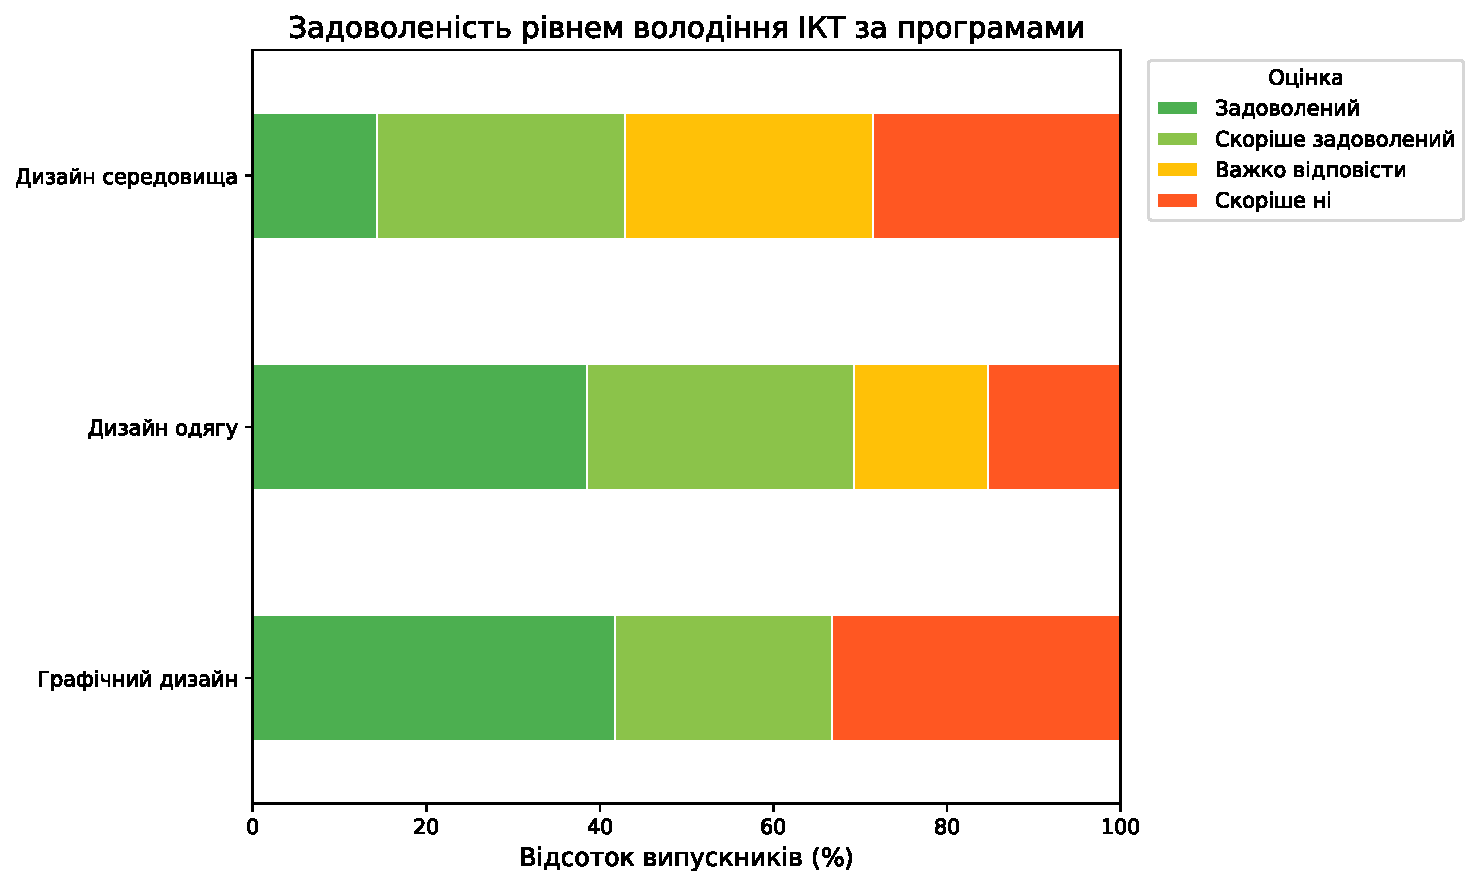
\includegraphics[width=0.9\textwidth]{figures/ikt_satisfaction_comparison.pdf}
    \caption{Задоволеність випускників рівнем володіння ІКТ за програмами}
    \label{fig:ikt-comparison}
\end{figure}

Серед дисциплін, названих випускниками як найважливіші та найкорисніші, переважають фахові практичні дисципліни: Композиція, Живопис, Рисунок, Комп'ютерні технології в дизайні. Випускники називають конкретне програмне забезпечення, яке потрібне на ринку праці: Adobe After Effects, Adobe Illustrator, Adobe Photoshop, Cinema 4D, Blender, Figma, 3ds Max, Archicad, AutoCAD, Revit, SketchUp. Примітно, що жоден випускник не згадав ШІ-інструменти, що може свідчити як про їх нерелевантність на момент навчання, так і про недостатню обізнаність.

\subsubsection{Аналіз опитування роботодавців}\label{sssec:2.2.4}

Опитано 9 роботодавців: ГД (5~осіб), ДО (2~особи), ДС (2~особи). Попри невеликий обсяг вибірки, результати містять якісно важливі дані.

\begin{figure}[htbp]
    \centering
    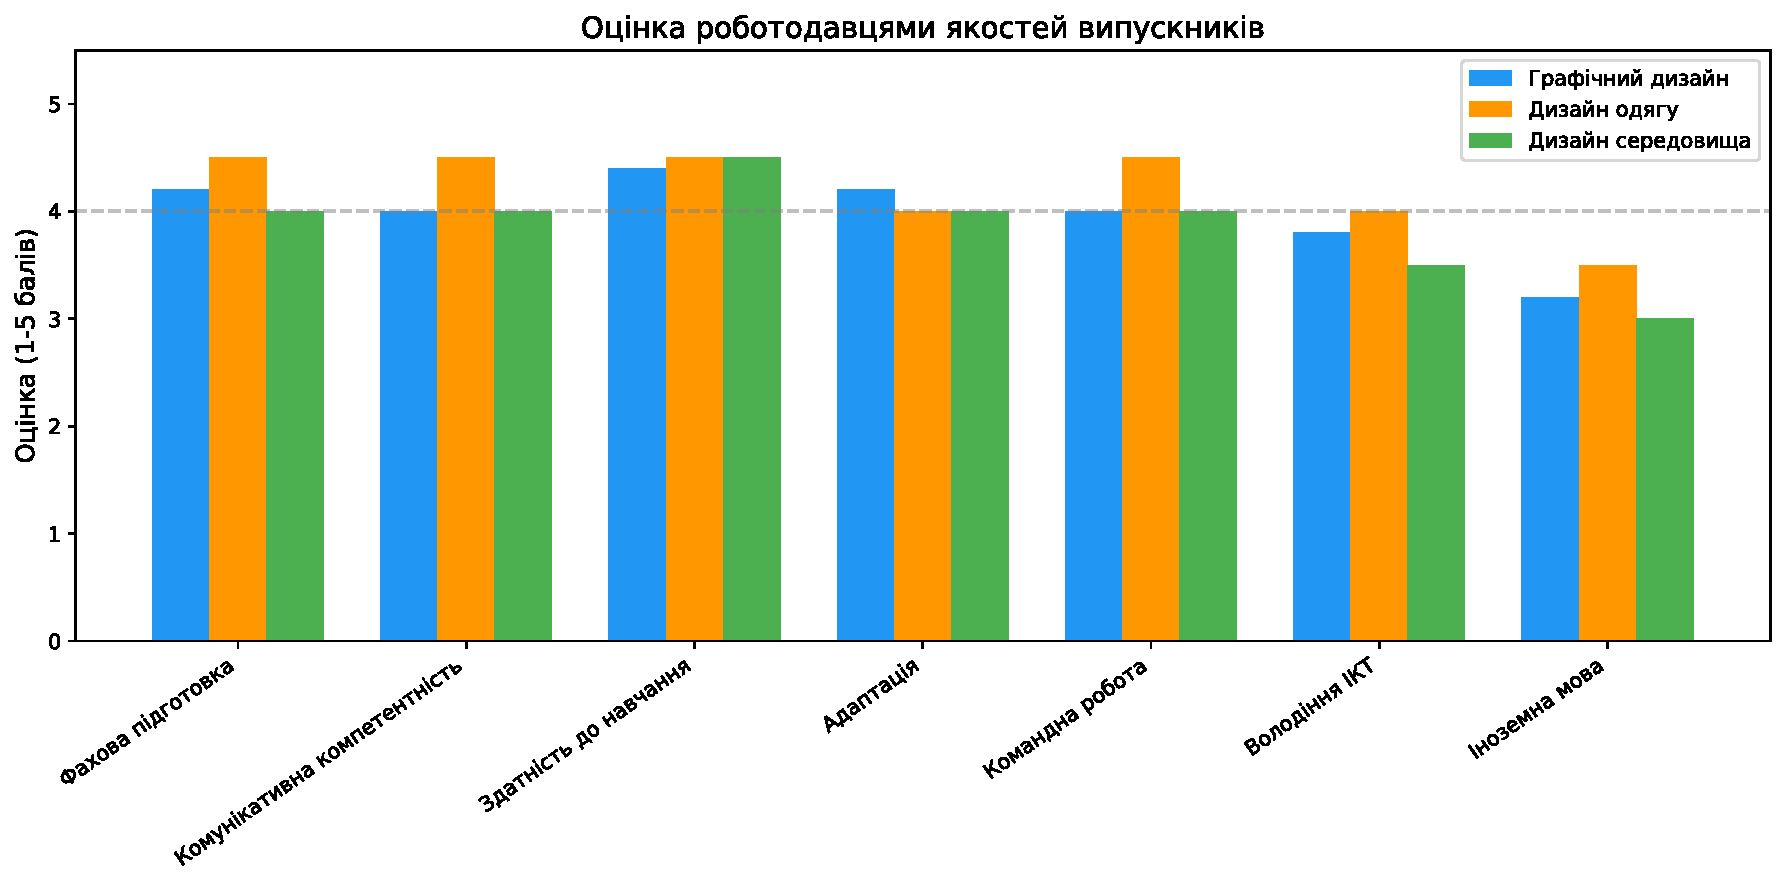
\includegraphics[width=0.95\textwidth]{figures/employer_quality_ratings.pdf}
    \caption{Оцінка роботодавцями якостей випускників (5-бальна шкала)}
    \label{fig:employer-quality}
\end{figure}

Ключові знахідки з опитування роботодавців:
\begin{enumerate}
    \item Оцінка \textbf{ІКТ-навичок} випускників коливається від 3,5 (ДС) до 4,0 (ДО) балів~--- нижче середнього порівняно з іншими якостями (рис.~\ref{fig:employer-quality});
    \item Знання \textbf{іноземної мови} має найнижчу оцінку (3,0--3,5), що обмежує доступ до міжнародних ШІ-ресурсів та документації;
    \item Роботодавці програми <<Дизайн одягу>> \textbf{прямо рекомендують інтеграцію ШІ}: <<Використання штучного інтелекту у сфері дизайну>>;
    \item Серед пріоритетів вдосконалення роботодавці виділяють: оновлення матеріально-технічної бази, збільшення обсягу практичної підготовки та зміни у змісті навчальних програм.
\end{enumerate}

\subsubsection{Аналіз опитування студентів (Moodle 2021)}\label{sssec:2.2.5}

Додатково проаналізовано дані масштабного опитування здобувачів освіти, проведеного через систему Moodle у лютому 2021~р. (61 респондент: ГД~--- 31, ДО~--- 12, ДС~--- 18, 50 питань). Для оцінки статистичної значущості міжпрограмних відмінностей застосовано критерій Краскела--Уолліса.

\begin{table}[htbp]
\centering
\caption{Результати порівняння програм за критерієм Краскела--Уолліса}\label{tab:kruskal-wallis}
\small
\begin{tabularx}{\textwidth}{@{}p{0.45\textwidth}rrr@{}}
\toprule
\textbf{Питання} & \textbf{$H$} & \textbf{$p$} & \textbf{Знач.} \\
\midrule
Матеріально-технічне забезпечення & 8,708 & 0,013 & Так \\
Інформаційне та навч.-метод. забезпечення & 6,019 & 0,049 & Так \\
Задоволеність рівнем знань та умінь & 5,495 & 0,064 & Ні \\
Професіоналізм викладачів & 4,218 & 0,121 & Ні \\
Студентоцентрованість & 3,720 & 0,156 & Ні \\
Індивідуальна освітня траєкторія & 3,347 & 0,188 & Ні \\
\bottomrule
\end{tabularx}
\end{table}

Статистично значущі відмінності ($p < 0{,}05$) виявлено за двома питаннями:
\begin{itemize}
    \item \textbf{Матеріально-технічне забезпечення} ($H = 8{,}708$, $p = 0{,}013$)~--- студенти ГД значно менш задоволені, ніж студенти ДО та ДС. Це пояснюється тим, що графічний дизайн більш залежний від комп'ютерного обладнання та програмного забезпечення;
    \item \textbf{Інформаційне та навчально-методичне забезпечення} ($H = 6{,}019$, $p = 0{,}049$)~--- знову ж, ГД демонструє найнижчу задоволеність, що корелює з більшою потребою у цифрових ресурсах.
\end{itemize}

Відповіді на відкриті питання підтверджують потребу в модернізації: студенти називають <<застаріле програмне забезпечення (Photoshop 2003)>>, <<старі комп'ютери>>, потребу у <<сучасних цифрових інструментах>> та <<більше практичної роботи з програмами>>.

\subsubsection{Аналіз висновків експертних груп НАЗЯВО}\label{sssec:2.2.6}

Проаналізовано висновки експертних груп НАЗЯВО для трьох програм КДПУ. Тематичне кодування за 5 категоріями (4 компоненти ІКК + загальна якість) виявило:

\begin{table}[htbp]
\centering
\caption{Тематичне кодування висновків експертних груп НАЗЯВО}\label{tab:expert-coding}
\small
\begin{tabularx}{\textwidth}{@{}Xrrr@{}}
\toprule
\textbf{Тематична категорія} & \textbf{ГД} & \textbf{ДО} & \textbf{ДС} \\
\midrule
Інформаційно-аналітичний & 114 & 101 & 108 \\
Комунікативний & 23 & 31 & 24 \\
Технологічний & 80 & 71 & 70 \\
Рефлексивний & 12 & 11 & 12 \\
Загальна якість & 199 & 212 & 194 \\
\bottomrule
\end{tabularx}
\end{table}

Висновки експертних груп демонструють порівняно рівномірний розподіл ІКК-тематики між програмами. Примітно, що рефлексивний компонент має найменше представництво (11--12 згадувань), що підтверджує його недостатню розвиненість у чинних програмах. Технологічний компонент (70--80 згадувань) представлений переважно через згадки комп'ютерного обладнання та програмного забезпечення, без ШІ-тематики.

\subsubsection{Синтез кейс-стаді КДПУ}\label{sssec:2.2.7}

Тріангуляція даних (ОПП, силабуси, опитування випускників, роботодавців, студентів, висновки НАЗЯВО) дозволяє сформулювати комплексну картину стану формування ІКК у КДПУ:

\begin{enumerate}
    \item \textbf{Нисхідний тренд ІКК-змісту}: кількість ІКК-ключових слів у ОПП зменшилась на 35\% (зі 122 до 75--82) між 2018 та 2021~рр.;
    \item \textbf{Нульове покриття ШІ}: жоден з 132 проаналізованих документів не містить термінів, пов'язаних із ШІ, генеративним дизайном або промпт-інженерією;
    \item \textbf{Незадоволеність випускників}: від 15,4\% до 33,3\% випускників не задоволені рівнем ІКТ-підготовки, причому найбільша незадоволеність~--- у програмі ГД;
    \item \textbf{Запит роботодавців}: пряма рекомендація інтеграції ШІ у навчання; найнижчі оцінки~--- ІКТ-навички та іноземна мова;
    \item \textbf{Статистично значущі відмінності}: ГД суттєво відрізняється від ДО та ДС за задоволеністю матеріально-технічним та інформаційним забезпеченням ($p < 0{,}05$);
    \item \textbf{Найбільша потреба}: графічний дизайн, як найбільш цифрово-залежна програма, демонструє найгострішу потребу у модернізації ІКК-змісту.
\end{enumerate}

Ці дані разом із загальнонаціональним аналізом (п.~\ref{subsec:2.1}) створюють обґрунтовану базу для розробки моделі трансформації навчальних програм (розділ~\ref{sec:3}).
